\section{Budget}
\label{sec:budget}

\subsection{Identification and Estimation of Costs}
\label{subsec:identification-estimation-costs}

The financial estimation of this project treats the thesis as a professional software engineering contract. To provide a highly realistic budget, all expenses are categorized into Direct Costs , Indirect Costs, and Contingencies.

Combining these categories, the total cost estimation can be expressed with the following formula:

\begin{equation}
Total\ Costs\ = Direct\ Costs + Indirect\ Costs + Contingency\ Costs
\end{equation}

\subsubsection{Direct Costs: Human Costs}
\label{subsubsec:direct-costs-human-costs}

Human resources constitute the primary direct cost of this project. There are three main agents that contribute to the execution and supervision of the thesis: the Thesis Director, Dr. Lluís Padró Cirera, the Project Management Tutor, Dr. Eduard Balbuena Longo, and the author of the thesis, Oriol Farrés i Vilar. 

Because each of these agents contributes to the project in fundamentally different ways, their costs are estimated based on their specific technical value. Furthermore, to accurately reflect the market value of the tasks performed, the thesis autor's workload is divided into four different roles. The roles the agents perform are detailed as follows:

\begin{itemize}
    \item \textbf{Advisory Board (Consulting Roles):}
    \begin{itemize}
        \item \textbf{Thesis Director -- Dr. Lluís Padró Cirera:} Provides high-level academic supervision and scientific validation. Responsible for guiding the overall architectural direction of the thesis.
        \item \textbf{Project Management Tutor -- Eduard Balbuena Longo:} Oversees the project management phase, ensuring adherence to UPC-FIB timelines.
    \end{itemize}
    
    \vspace{0.5em}
    \item \textbf{Execution Team (Principal Developer): Oriol Farrés i Vilar}. \\
    To accurately reflect the diverse technical and administrative demands of the project, the principal developer's workload is divided into four highly specialized roles:
    \begin{itemize}
        \item \textbf{Project Manager:} Handles day-to-day Agile sprint tracking, resource allocation, Earned Value Management (EVM) cost control, and active risk mitigation.
        \item \textbf{R\&D Engineer:} Leads the theoretical research and algorithm design, specifically focusing on the Choquet integral mathematics, theoretical bounds, and fine-tuning strategies.
        \item \textbf{AI Systems Engineer:} Executes the high-performance engineering tasks, including the C++ solver implementation, hardware optimization, and architecture design for the AI infrastructure.
        \item \textbf{Documentation Engineer:} Dedicated strictly to the technical redaction of the project, including end-of-sprint statistical reporting, thesis formatting, and defense preparation.
    \end{itemize}
\end{itemize}

\paragraph{Labor Rate Calculation Methodology}
To estimate the true corporate cost of these human resources, this budget utilizes the \textbf{Fully Burdened Labor Rate}. This method accounts for the actual cost to the employer, comprising not only the gross salary but also a mandatory \textbf{1.35 multiplier}. This markup accurately absorbs the Spanish statutory employer Social Security contributions \cite{boe_cotizacion_2024}.

The base hourly cost is inferred by dividing the Yearly Gross Salary by the legally mandated annual working hours.

\begin{equation}
    \text{Base Hourly Cost} = \frac{\text{Yearly Gross Salary}}{\text{Annual Working Hours}}
\end{equation}

In Spain, while the Workers' Statute establishes an absolute legal maximum of 1,826 hours and 27 minutes, the actual yearly hours worked vary significantly depending on the sector's specific collective agreement, typically ranging between 1,740 and 1,800 hours per year \cite{estatuto_trabajadores}. For the specific scope of this project, the calculations strictly adhere to the \textit{Convenio Colectivo de Empresas de Consultoría y Tecnologías de la Información (TIC)}, which establishes a maximum annual working calendar of \textbf{1,800 hours} for software engineering and IT professionals \cite{convenio_tic_2023}. 

Consequently, the proper computation for the project's financial estimation follows this exact formula:
\begin{equation}
    \text{Total Hourly Cost} = \left( \frac{\text{Yearly Gross Salary}}{1800} \right) \times 1.35
\end{equation}


Let us now apply these rates to the exact hour allocation for each role, as defined in the project planning phase.

\begin{table}[H]
\centering
\caption{Task summary mapping the exact hour distribution across the six specialized human resource roles. The total comprises 540 execution hours and 40 consulting hours.}
\label{tab:task-summary-roles}
\resizebox{\textwidth}{!}{%
\begin{tabular}{llcccccc|c}
\rowcolor[HTML]{34495E} 
{\color[HTML]{FFFFFF} \textbf{ID}} & {\color[HTML]{FFFFFF} \textbf{Task Name}} & {\color[HTML]{FFFFFF} \textbf{Dir.}} & {\color[HTML]{FFFFFF} \textbf{Tut.}} & {\color[HTML]{FFFFFF} \textbf{PM}} & {\color[HTML]{FFFFFF} \textbf{R\&D}} & {\color[HTML]{FFFFFF} \textbf{AI Sys.}} & {\color[HTML]{FFFFFF} \textbf{Doc.}} & {\color[HTML]{FFFFFF} \textbf{Total (h)}} \\ 
\rowcolor[HTML]{D5D8DC} 
\multicolumn{9}{l}{\textbf{Sprint 0: Project Management}} \\ 
PM.1 & ICT Tools Study & - & - & 4.00 & - & - & - & 4.00 \\ 
PM.2 & Context and Scope & - & - & 24.50 & - & - & - & 24.50 \\ 
PM.3 & Project Planning & - & - & 8.25 & - & - & - & 8.25 \\ 
PM.4 & Budget and Sustainability & - & - & 9.25 & - & - & - & 9.25 \\ 
PM.5 & Personal and Prof. Skills & - & - & 6.25 & - & - & - & 6.25 \\ 
PM.6 & Integration in Final Doc & - & 10.00 & 18.25 & - & - & - & 28.25 \\ 
PM.7 & Supervisor Meetings & 19.50 & - & 19.50 & - & - & - & 39.00 \\ 
\rowcolor[HTML]{D6EAF8} 
\multicolumn{9}{l}{\textbf{Sprint 1: Research, Learning \& Baseline}} \\ 
PH0.1 & Adv. C++ \& Lit Review & - & - & - & 20.00 & - & - & 20.00 \\ 
PH0.2a & Naive Retrieval Setup & - & - & - & - & 15.00 & - & 15.00 \\ 
PH0.2b & Base Generation \& Eval & - & - & - & - & 15.00 & - & 15.00 \\ 
PH0.3 & Baseline Documentation & - & - & - & - & - & 10.00 & 10.00 \\ 
\rowcolor[HTML]{AED6F1} 
\multicolumn{9}{l}{\textbf{Sprint 2: Game-Theoretic Subset Optimization}} \\ 
PH1.1 & Simple Reranking & - & - & - & 15.00 & - & - & 15.00 \\ 
PH1.2 & Choquet via GA & - & - & - & 20.00 & - & - & 20.00 \\ 
PH1.3a & B\&B Algorithm Design & - & - & - & 15.00 & - & - & 15.00 \\ 
PH1.3b & B\&B C++ Execution & - & - & - & - & 20.00 & - & 20.00 \\ 
PH1.4 & PH1 Documentation & - & - & - & - & - & 10.00 & 10.00 \\ 
\rowcolor[HTML]{D6EAF8} 
\multicolumn{9}{l}{\textbf{Sprint 3: Role-Conditioned Alignment}} \\ 
PH2.1 & OD to SD Pipeline & - & - & - & - & 15.00 & - & 15.00 \\ 
PH2.2 & SD Generation & - & - & - & - & 15.00 & - & 15.00 \\ 
PH2.3 & ORPO Fine-Tuning & - & - & - & 15.00 & - & - & 15.00 \\ 
PH2.4 & QDORA Implementation & - & - & - & - & 25.00 & - & 25.00 \\ 
PH2.5 & PH2 Documentation & - & - & - & - & - & 10.00 & 10.00 \\ 
\rowcolor[HTML]{AED6F1} 
\multicolumn{9}{l}{\textbf{Sprint 4: Hardware-Efficient Execution}} \\ 
PH3.1 & S-QDORA Architecture & - & - & - & - & 20.00 & - & 20.00 \\ 
PH3.2 & Speculative Decoding & - & - & - & 15.00 & - & - & 15.00 \\ 
PH3.3 & Hardware Management & - & - & - & - & 15.00 & - & 15.00 \\ 
PH3.4 & End-to-End Orchestration & - & - & - & - & 20.00 & - & 20.00 \\ 
PH3.5 & PH3 Documentation & - & - & - & - & - & 10.00 & 10.00 \\ 
\rowcolor[HTML]{D6EAF8} 
\multicolumn{9}{l}{\textbf{Sprint 5: Statistical Benchmark \& Validation}} \\ 
PH4.1 & Local Evaluator Deploy & - & - & - & - & 20.00 & - & 20.00 \\ 
PH4.2 & Metaheuristic Judge & - & - & - & 25.00 & - & - & 25.00 \\ 
PH4.3a & VRAM Tier Config & - & - & - & - & 20.00 & - & 20.00 \\ 
PH4.3b & Hardware Ablation Exec. & - & - & - & - & 15.00 & - & 15.00 \\ 
PH4.4 & PH4 Documentation & - & - & - & - & - & 10.00 & 10.00 \\ 
\rowcolor[HTML]{AED6F1} 
\multicolumn{9}{l}{\textbf{Sprint 6: Final Documentation \& Defense}} \\ 
DOC.1 & Thesis Redaction & - & - & - & - & - & 40.00 & 40.00 \\ 
DOC.2 & Defense Preparation & 10.50 & - & 20.00 & - & - & - & 30.50 \\ \hline
\rowcolor[HTML]{34495E} 
\multicolumn{2}{r}{{\color[HTML]{FFFFFF} \textbf{Total Hours by Role}}} & {\color[HTML]{FFFFFF} \textbf{30.00}} & {\color[HTML]{FFFFFF} \textbf{10.00}} & {\color[HTML]{FFFFFF} \textbf{110.00}} & {\color[HTML]{FFFFFF} \textbf{125.00}} & {\color[HTML]{FFFFFF} \textbf{215.00}} & {\color[HTML]{FFFFFF} \textbf{90.00}} & {\color[HTML]{FFFFFF} \textbf{580.00}} \\ \hline
\end{tabular}%
}
\source{Compiled by the author}
\end{table}


Let us now calculate the Fully Burdened Labor Rate for each role.

\begin{table}[H]
\centering
\caption{Calculation of the Fully Burdened Labor Rate based on 1,800 annual working hours and a 1.35 Social Security multiplier for the 2026 fiscal year.}
\label{tab:human-resource-rates}
\resizebox{\textwidth}{!}{%
\begin{tabular}{lcccc}
\rowcolor[HTML]{34495E} 
{\color[HTML]{FFFFFF} \textbf{Role}} & {\color[HTML]{FFFFFF} \textbf{Yearly Gross (€)}} & {\color[HTML]{FFFFFF} \textbf{Base Hourly Cost (€/h)}} & {\color[HTML]{FFFFFF} \textbf{Social Security (+35\%)}} & {\color[HTML]{FFFFFF} \textbf{Total Hourly Cost (€/h)}} \\ 
\rowcolor[HTML]{D5D8DC} 
\multicolumn{5}{l}{\textbf{Advisory Board (Consulting Costs)}} \\ 
Thesis Director & 74,000.00 \cite{upc_retribuciones_2026} & 41.11 & 14.39 & \textbf{55.50} \\ 
Project Management Tutor & 63,000.00 \cite{upc_retribuciones_2026} & 35.00 & 12.25 & \textbf{47.25} \\ 
\rowcolor[HTML]{D6EAF8} 
\multicolumn{5}{l}{\textbf{Execution Team (Principal Developer)}} \\ 
R\&D Engineer & 52,000.00 \cite{hays_salary_guide_2026, michael_page_2026} & 28.89 & 10.11 & \textbf{39.00} \\ 
Project Manager & 48,000.00 \cite{hays_salary_guide_2026} & 26.67 & 9.33 & \textbf{36.00} \\ 
AI Systems Engineer & 48,000.00 \cite{hays_salary_guide_2026, michael_page_2026} & 26.67 & 9.33 & \textbf{36.00} \\ 
Documentation Eng. & 32,000.00 \cite{hays_salary_guide_2026} & 17.78 & 6.22 & \textbf{24.00} \\ \hline
\end{tabular}%
}
\source{Compiled by the author}
\end{table}






With the precise allocation of hours established for each specific role in Table \ref{tab:task-summary-roles}, the total direct human costs can now be accurately computed. By multiplying the total hours dedicated to each profile by their respective fully burdened labor rates (previously defined in Table \ref{tab:human-resource-rates}), we obtain the final financial requirement for the project's workforce. 

The following table summarizes these calculations, aggregating the 540 execution hours and the 40 consulting hours into a definitive total direct cost.

\begin{table}[H]
\centering
\caption{Final calculation of the Direct Costs, combining the established hourly rates with the exact hour allocation per role.}
\label{tab:total-direct-costs}
\resizebox{0.85\textwidth}{!}{%
\begin{tabular}{lccc}
\rowcolor[HTML]{34495E} 
{\color[HTML]{FFFFFF} \textbf{Resource / Role}} & {\color[HTML]{FFFFFF} \textbf{Total Hours}} & {\color[HTML]{FFFFFF} \textbf{Rate (€/h)}} & {\color[HTML]{FFFFFF} \textbf{Total Cost (€)}} \\ 
\rowcolor[HTML]{D5D8DC} 
\multicolumn{4}{l}{\textbf{Advisory Board (Consulting Roles)}} \\ 
Thesis Director & 30.00 & 55.50 & 1,665.00 \\ 
Project Management Tutor & 10.00 & 47.25 & 472.50 \\ 
\rowcolor[HTML]{D6EAF8} 
\multicolumn{4}{l}{\textbf{Execution Team (Principal Developer)}} \\ 
AI Systems Engineer & 215.00 & 36.00 & 7,740.00 \\ 
R\&D Engineer & 125.00 & 39.00 & 4,875.00 \\ 
Project Manager & 110.00 & 36.00 & 3,960.00 \\ 
Documentation Engineer & 90.00 & 24.00 & 2,160.00 \\ \hline
\rowcolor[HTML]{2C3E50} 
{\color[HTML]{FFFFFF} \textbf{TOTAL DIRECT COSTS}} & {\color[HTML]{FFFFFF} \textbf{580.00}} & {\color[HTML]{FFFFFF} \textbf{---}} & {\color[HTML]{FFFFFF} \textbf{20,977.50 €}} \\ \hline
\end{tabular}%
}
\source{Compiled by the author}
\end{table}

As reflected in Table \ref{tab:total-direct-costs}, the absolute total for the Direct Costs of this thesis amounts to \textbf{20,977.50 \euro}. 



\subsubsection{Indirect Costs}
\label{subsubsec:indirect-costs}

\paragraph{1. Hardware Amortization}
The physical infrastructure relies on a localized high-performance workstation. To optimize CAPEX, the core server components were strategically procured in November 2025 (Q4), taking advantage of end-of-year supplier liquidations to hedge against the projected Q1 2026 RAM inflation. 

Table \ref{tab:hardware-costs} details the exact prices paid for each component required to assemble the Deep Learning server.

\begin{table}[H]
\centering
\caption{Breakdown of the high-performance local server components 
procured for the project. Prices include IVA at the statutory Spanish 
rate of 21\%, as this reflects the true capital expenditure incurred 
and constitutes the correct amortization base under AEAT guidelines.}
\label{tab:hardware-costs}
\resizebox{0.85\textwidth}{!}{%
\begin{tabular}{llc}
\rowcolor[HTML]{34495E} 
{\color[HTML]{FFFFFF} \textbf{Component}} & {\color[HTML]{FFFFFF} \textbf{Hardware Name}} & {\color[HTML]{FFFFFF} \textbf{Price (incl. IVA 21\%, €)}} \\ 
\rowcolor[HTML]{D5D8DC} 
CPU & Ryzen 9 9900x & 371.91 \\ 
GPUs & 3090 GigaByte (2 uds) & 1,399.99 \\ 
\rowcolor[HTML]{D5D8DC} 
PSUs & Corsair Platinum HX1200 (2 uds) & 180.00 \\ 
Motherboard & ASUS ProArt X870E-CREATOR WIFI & 419.91 \\ 
\rowcolor[HTML]{D5D8DC} 
Chassis & Fractal Design Torrent & 198.90 \\ 
CPU cooler & Phantom Spirit 120 SE & 39.59 \\ 
\rowcolor[HTML]{D5D8DC} 
RAM & Corsair Vengeance DDR5 2x24GB 6000MHz CL36 & 203.98 \\ 
Storage & 1TB SSD 7250MB/s & 79.55 \\ 
\rowcolor[HTML]{D5D8DC} 
Riser Cable 4.0 & AVA PCIe 4.0 Gen 4 x 16 & 55.49 \\ \hline
\rowcolor[HTML]{2C3E50} 
\multicolumn{2}{r}{{\color[HTML]{FFFFFF} \textbf{TOTAL HARDWARE PRICE}}} & 
{\color[HTML]{FFFFFF} \textbf{2,949.31}} \\ \hline
\end{tabular}%
}
\source{Compiled by the author}
\end{table}

With the total acquisition cost established, we must calculate the amortization cost for the duration of the project. For the amortization of IT hardware, the Spanish Tax Agency (AEAT) allows for a maximum linear coefficient of 25\% annually, which corresponds to a 4-year lifecycle. Given that the project duration is 4.5 months, we calculate the proportional depreciation for that specific period using the following formula:

\begin{equation}
\text{HW Amortization} = \text{HW Cost} \times \text{Annual Depreciation Rate} \times \left( \frac{\text{Project Duration}}{12} \right)
\end{equation}

Which translates to:

\begin{equation}
\text{HW Amortization} = 2,949.31 \, \text{\euro} \times 0.25 \times \left( \frac{4.5}{12} \right) = \textbf{276.50 \euro}
\end{equation}


\paragraph{2. Software Costs: Zero-Cost Strategy}
A core financial directive of this thesis is the absolute minimization of recurring software licensing (OPEX). The project achieves a \textbf{0.00 €} software budget by strictly utilizing enterprise-grade open-source frameworks. The operating system (Kubuntu 24.04), AI orchestration libraries (PyTorch, vLLM, HuggingFace), and the foundational models themselves (Llama-3, DeepSeek) operate under permissive open-source licenses. 

As all software components are open-source and carry no licensing
fee, no IVA liability arises for this category.

For completeness, the following additional indirect cost categories are
acknowledged and formally justified as zero-cost items: \textbf{software
maintenance} incurs no cost as all frameworks are community-maintained
under open-source licenses with no paid support contracts;
\textbf{hardware repair and replacement} is covered by the contingency
reserve provisioned in Section~\ref{subsubsec:contingency-costs-unforeseen-costs}
and requires no separate budget line; \textbf{cloud backup and storage}
incurs no cost as all data, models, and checkpoints are stored exclusively
on the local 1TB NVMe drive and the DECFA internal network, consistent
with the project's strict no-cloud-API constraint.

\paragraph{3. Facilities, Electricity, and Connectivity}
The operational environment is provided by \textit{Decolletatge Farrés S.A.} (DECFA), an industrial manufacturing firm, which has allocated a 20 $\text{m}^2$ corporate office space for the duration of the project. While provided internally, these resources must be accounted for at market rates to reflect the true autonomous cost of the project.

\begin{itemize}
    \item \textbf{Office Space (Work Zone):} The allocated space is valued at an industrial standard rate of 10.00 \euro/$\text{m}^2$/month. Over the 4.5-month project lifecycle, the equivalent facility cost is calculated as:
    \begin{equation}
        \text{Work Zone Cost} = 20 \, \text{m}^2 \times 10.00 \, \frac{\text{\euro}}{\text{m}^2 \cdot \text{month}} \times 4.5 \, \text{months} = \textbf{900.00 \euro}
    \end{equation}

    Office space is provided internally by DECFA at market rates for 
accounting purposes; as an intra-company allocation, no IVA 
transaction is generated.

    \item \textbf{Industrial Connectivity (WiFi / Fiber):} The facility utilizes an enterprise-grade fiber optic connection costing 150.00 \euro/month. It would be an accounting error to allocate the entirety of this corporate overhead to a single project. Based on a 24-hour network telemetry test conducted during a standard workday, the workstation and cloud API calls utilized approximately 2,46\% of the total company bandwidth. Therefore, the prorated cost is:
    \begin{equation}
        \text{Connectivity Cost} = 150.00 \, \frac{\text{\euro}}{\text{month}} \times 0.0246 \times 4.5 \, \text{months} = \textbf{16.47 \euro}
    \end{equation}

    The connectivity cost represents a prorated share of DECFA's 
corporate fiber contract; IVA is absorbed by the company as a 
registered VAT entity and is therefore excluded from the project 
cost allocation.

    \item \textbf{Electricity Consumption:} The localized AI training approach is highly energy-intensive. To accurately reflect the power draw, the consumption is divided into two distinct profiles. The nominal 540 project hours are calculated at a standard operational draw of 0.30 kW\footnote{Empirical measurement taken at the wall using a Wattmeter during a standard 8-hour development and documentation session, where GPUs remained primarily in idle states.}, while an estimated 300 hours of unmonitored overnight GPU execution (e.g., ORPO alignment algorithms and hardware ablation tests) are calculated at a peak draw of 0.85 kW\footnote{Empirical measurement recorded during a sustained multi-hour ORPO fine-tuning epoch, fully saturating the Dual RTX 3090 VRAM and CUDA cores alongside the Ryzen 9 CPU.
These 300 hours correspond to overnight training runs scheduled in
Sprints~3 and~5 (tasks PH2.3, PH2.4, and PH4.3b), which execute
outside nominal working hours to avoid blocking the development
workstation during the day.}. Importantly, DECFA operates under a closed-contract industrial electricity rate of 0.16 \euro/kWh, entirely shielding the project from spot market volatility. The total energy cost is computed as the sum of both workloads:
    
    \begin{equation}
        \begin{split}
            \text{Electricity Cost} &= \left( 540 \, \text{h} \times 0.30 \, \text{kW} \times 0.16 \, \frac{\text{\euro}}{\text{kWh}} \right) \\
            &\quad + \left( 300 \, \text{h} \times 0.85 \, \text{kW} \times 0.16 \, \frac{\text{\euro}}{\text{kWh}} \right)
        \end{split}
    \end{equation}
    \begin{equation*}
        \text{Electricity Cost} = 25.92 \, \text{\euro} + 40.80 \, \text{\euro} = \textbf{66.72 \euro}
    \end{equation*}

    Electricity is billed under DECFA's industrial closed-contract 
rate, which is VAT-inclusive at the corporate level; the per-kWh 
rate of 0.16~\euro\ used here reflects the net cost allocated to 
the project.
\end{itemize}

\paragraph{4. Logistical and Transportation Costs}
Physical commutes to the \textit{Decolletatge Farrés S.A.} facility for daily project execution are calculated based on exact fuel consumption. The route constitutes a 5.5 km urban trajectory from the author's residence to the workspace and an optimized 4.3 km return route, totaling 9.8 km per round trip.
Daily physical presence at the DECFA facility is a strict operational
requirement, as all GPU-dependent training and inference tasks execute
on the on-premise workstation and cannot be performed remotely without
violating the project's data privacy constraints.
The designated vehicle, an Opel Corsa, has an empirically compiled urban consumption rate of 7.2 L/100 km.

Assuming a daily commute (5 days a week) over the 18-week project span, the total number of round trips is 90, resulting in a cumulative distance of 882 km. With an average projected  fuel cost of 1.65 \euro/L\footnote{This projected cost might be too optimistic given the global context we are currently presencing.}, the transportation expense is mathematically defined as:

\begin{equation}
\text{Total Distance} = 90 , \text{trips} \times (5.5 , \text{km} + 4.3 , \text{km}) = 882 , \text{km}
\end{equation}

\begin{equation}
\text{Transport Cost} = \left( \frac{882 , \text{km} \times 7.2 , \text{L}}{100 , \text{km}} \right) \times 1.65 , \frac{\text{\euro}}{\text{L}} = \textbf{104.78 \euro}
\end{equation}

Fuel costs are calculated at the pump price inclusive of all applicable
taxes; no separate IVA adjustment is required.



\subsubsection*{Summary of Indirect Costs}

Table \ref{tab:indirect-costs-summary} aggregates all the previously calculated indirect operational expenses, including hardware depreciation, facility usage, and logistics, necessary for the execution of the project.

\begin{table}[H]
\centering
\caption{Aggregate summary of all indirect costs associated with hardware depreciation, facility usage, and logistics.}
\label{tab:indirect-costs-summary}
\begin{tabular}{lc}
\rowcolor[HTML]{34495E} 
{\color[HTML]{FFFFFF} \textbf{Concept}} & {\color[HTML]{FFFFFF} \textbf{Cost (€)}} \\ 
\rowcolor[HTML]{D5D8DC} 
Hardware Costs & 276.50 \\ 
Software Costs & 0.00 \\ 
\rowcolor[HTML]{D5D8DC} 
Office Costs & 900.00 \\ 
WiFi Costs & 16.47 \\ 
\rowcolor[HTML]{D5D8DC} 
Electricity Costs & 66.72 \\ 
Transportation Costs & 104.78 \\ \hline
\rowcolor[HTML]{2C3E50} 
{\color[HTML]{FFFFFF} \textbf{TOTAL INDIRECT COSTS}} & {\color[HTML]{FFFFFF} \textbf{1,364.47}} \\ \hline
\end{tabular}%
\source{Compiled by the author}
\end{table}

\subsubsection{Contingency Costs: Unforeseen Costs}
\label{subsubsec:contingency-costs-unforeseen-costs}

In highly experimental IT and AI infrastructure projects, financial deviations are not merely possible; they are statistically probable. To ensure the financial resilience of the thesis, the risk budget is strictly bifurcated according to Project Management Institute (PMI) standards into a generic management reserve and a specific contingency reserve based on Expected Monetary Value (EMV) \cite{pmbok_guide}.

\textbf{Generic Buffer (Management Reserve)}

The generic buffer serves as a Management Reserve to absorb \textit{unknown unknowns}—unforeseeable macroeconomic shifts, sudden supply chain hardware failures, or deprecation of open-source libraries that require architectural pivots. 

Standard corporate R\&D budgeting allocates between 10\% and 15\% for this reserve. For this project, a conservative \textbf{10\% flat rate} is applied to the sum of all accumulated Direct and Indirect Costs. Utilizing the baseline Direct Human Cost of exactly 20,977.50 \euro\ and an
Indirect Cost of 1,364.47 \euro\ (Total Baseline: 22,341.97 \euro), the
generic buffer is calculated as:

\begin{equation}
    \text{Generic Buffer} = 22,341.97 \, \text{\euro} \times 0.10 = \textbf{2,234.20 \euro}
\end{equation}

\textbf{Incidentals (Contingency Reserve)}

Unlike the generic buffer, incidentals account for \textit{known unknowns}—specific technical risks that were formally identified and quantified during the project planning phase (Deliverables 1 and 2). 

To calculate this, the budget utilizes the \textbf{Expected Monetary Value (EMV)} formula, which mathematically limits financial exposure based on the exact probability of a risk occurring \cite{pmbok_guide}.

\begin{equation}
    \text{EMV} = \text{Probability (\%)} \times \text{Financial Impact (\euro)}
\end{equation}

The three primary identified risks are provisioned as follows using the 2026 Fully Burdened Labor Rates defined in Table \ref{tab:human-resource-rates}:

\begin{itemize}
    \item \textbf{Risk 1: Branch \& Bound Solver Timeout.} \\
    \textit{Scenario:} The C++ exact solver exceeds the $T_1 < T_2$ latency constraints. \\
    \textit{Impact:} Requires an estimated 15 additional hours of the AI Systems Engineer (36.00 \euro/h) to implement a heuristic fallback. Total Impact: 540.00 \euro. \\
    \textit{Probability:} 30\%. \\
    \textit{Justification:} Branch \& Bound worst-case behaviour on adversarial
inputs is a documented risk in combinatorial optimization
literature~\cite{pmbok_guide}; a 30\% estimate reflects medium likelihood
given the 50ms hard constraint and the NP-hard search space of $\binom{64}{8}$. \\
    \textit{EMV Provision:} $540.00 \times 0.30 =$ \textbf{162.00 \euro}.

    \item \textbf{Risk 2: ORPO/GRPO Alignment Collapse.} \\
    \textit{Scenario:} The local foundational model overfits during preference alignment, degrading its reasoning capabilities. \\
    \textit{Impact:} Requires 25 additional hours of the R\&D Engineer (39.00 \euro/h) to reconstruct the dataset and tune hyperparameters. Total Impact: 975.00 \euro. \\
    \textit{Probability:} 20\%. \\
    \textit{Justification:} Alignment collapse probability is estimated at 20\%
based on analogous ORPO fine-tuning instability rates reported in
preference optimization literature, mitigated by the use of a well-validated
synthetic dataset construction pipeline. \\
    \textit{EMV Provision:} $975.00 \times 0.20 =$ \textbf{195.00 \euro}.

    \item \textbf{Risk 3: VRAM Overflow during 70B Judge Deployment.} \\
    \textit{Scenario:} The Dual RTX 3090 setup runs out of memory during the metaheuristic benchmarking phase. \\
    \textit{Impact:} Requires 10 additional hours of the AI Systems Engineer (36.00 \euro/h) to implement more aggressive 4-bit quantization and tensor parallelism adjustments. Total Impact: 360.00 \euro. \\
    \textit{Probability:} 40\%. \\
    \textit{Justification:} A 40\% probability reflects the high likelihood of
memory pressure when co-hosting a 70B evaluator and the inference pipeline
on a fixed 48GB VRAM envelope, a configuration that operates near the
theoretical memory ceiling under tensor parallelism. \\
    \textit{EMV Provision:} $360.00 \times 0.40 =$ \textbf{144.00 \euro}.
\end{itemize}


\begingroup
\definecolor{RiskHeader}{RGB}{52, 73, 94}   % Dark Blue as used previously
\definecolor{RiskLow}{RGB}{169, 223, 191}    % Light Green
\definecolor{RiskMedium}{RGB}{249, 231, 159} % Light Yellow
\definecolor{RiskHigh}{RGB}{250, 215, 160}   % Light Orange

\begin{figure}[H]
    \centering
    \includegraphics[width=0.8\textwidth]{images/risk-matrix.pdf} % Replaced tikz with a placeholder if needed or keeping tikz if requested, but instructions were for figures generally. Wait, I will keep the tikz and add \source. Actually, looking at the user request, it's about \source. I'll add \source to the figure environment.
    \caption{Project Management Risk Matrix visualization (Impact vs. Probability). Identifies the position of quantified \textit{Known-Unknown} technical risks within the stylized risk zones.}
    \label{fig:risk-matrix}
    \vspace{1em}
    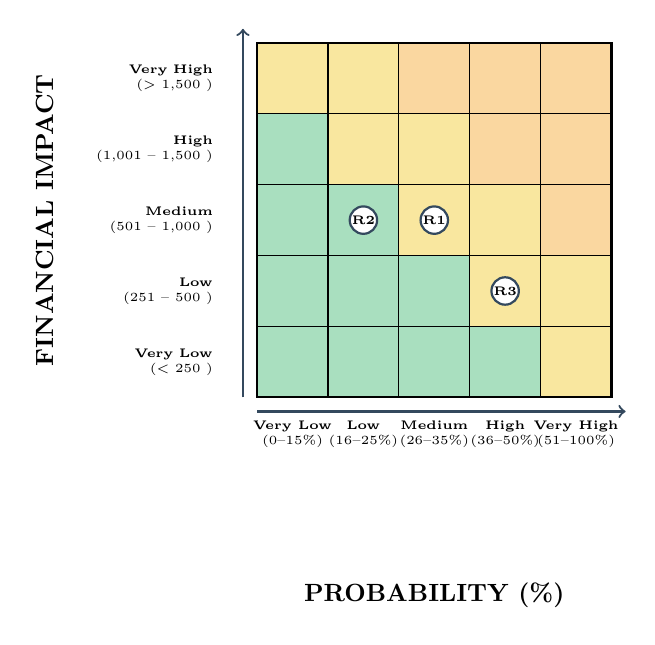
\begin{tikzpicture}[scale=0.9, transform shape]
        % Axes Labels
        \node[rotate=90, font=\bfseries] at (-3, 2.5) {FINANCIAL IMPACT};
        \node[below, font=\bfseries] at (2.5, -2.5) {PROBABILITY (\%)};

        % Category Labels (Impact)
        \node[left, align=right, font=\tiny, text width=2cm] at (-0.5, 4.5) {\textbf{Very High}\\(> 1,500 \euro)};
        \node[left, align=right, font=\tiny, text width=2cm] at (-0.5, 3.5) {\textbf{High}\\(1,001 -- 1,500 \euro)};
        \node[left, align=right, font=\tiny, text width=2cm] at (-0.5, 2.5) {\textbf{Medium}\\(501 -- 1,000 \euro)};
        \node[left, align=right, font=\tiny, text width=2cm] at (-0.5, 1.5) {\textbf{Low}\\(251 -- 500 \euro)};
        \node[left, align=right, font=\tiny, text width=2cm] at (-0.5, 0.5) {\textbf{Very Low}\\(< 250 \euro)};

       % Category Labels (Probability)
        \node[below, align=center, font=\tiny, yshift=-3pt] at (0.5, -0.1) {\textbf{Very Low}\\(0--15\%)};
        \node[below, align=center, font=\tiny, yshift=-3pt] at (1.5, -0.1) {\textbf{Low}\\(16--25\%)};
        \node[below, align=center, font=\tiny, yshift=-3pt] at (2.5, -0.1) {\textbf{Medium}\\(26--35\%)};
        \node[below, align=center, font=\tiny, yshift=-3pt] at (3.5, -0.1) {\textbf{High}\\(36--50\%)};
        \node[below, align=center, font=\tiny, yshift=-3pt] at (4.5, -0.1) {\textbf{Very High}\\(51--100\%)};

        % Background Color Fills for Risk Zones (Green: Low, Yellow: Medium, Orange: High)
        % Row VH (> 1500)
        \fill[RiskHigh] (4,4) rectangle (5,5);   % VH, VH
        \fill[RiskHigh] (3,4) rectangle (4,5);   % VH, H
        \fill[RiskHigh] (2,4) rectangle (3,5);   % VH, M
        \fill[RiskMedium] (1,4) rectangle (2,5); % VH, L
        \fill[RiskMedium] (0,4) rectangle (1,5); % VH, VL

        % Row H (1001-1500)
        \fill[RiskHigh] (4,3) rectangle (5,4);   % H, VH
        \fill[RiskHigh] (3,3) rectangle (4,4);   % H, H
        \fill[RiskMedium] (2,3) rectangle (3,4); % H, M
        \fill[RiskMedium] (1,3) rectangle (2,4); % H, L
        \fill[RiskLow] (0,3) rectangle (1,4);    % H, VL

        % Row M (501-1000) - R1 (30% M Prob, 540e M Imp)
        \fill[RiskHigh] (4,2) rectangle (5,3);   % M, VH
        \fill[RiskMedium] (3,2) rectangle (4,3); % M, H
        \fill[RiskMedium] (2,2) rectangle (3,3); % M, M - R1 lands here
        \fill[RiskLow] (1,2) rectangle (2,3);    % M, L
        \fill[RiskLow] (0,2) rectangle (1,3);    % M, VL

        % Row L (251-500) - R2 (20% L Prob, 975e M-H Imp -> categorised M), R3 (40% H Prob, 360e L Imp)
        \fill[RiskMedium] (4,1) rectangle (5,2); % L, VH
        \fill[RiskMedium] (3,1) rectangle (4,2); % L, H - R3 lands here
        \fill[RiskLow] (2,1) rectangle (3,2);    % L, M
        \fill[RiskLow] (1,1) rectangle (2,2);    % L, L - R2 lands here
        \fill[RiskLow] (0,1) rectangle (1,2);    % L, VL

        % Row VL (< 250)
        \fill[RiskMedium] (4,0) rectangle (5,1); % VL, VH
        \fill[RiskLow] (3,0) rectangle (4,1);    % VL, H
        \fill[RiskLow] (2,0) rectangle (3,1);    % VL, M
        \fill[RiskLow] (1,0) rectangle (2,1);    % VL, L
        \fill[RiskLow] (0,0) rectangle (1,1);    % VL, VL

        % Draw main grid lines
        \draw[thick] (0,0) rectangle (5,5);
        \draw (1,0) -- (1,5); \draw (2,0) -- (2,5); \draw (3,0) -- (3,5); \draw (4,0) -- (4,5);
        \draw (0,1) -- (5,1); \draw (0,2) -- (5,2); \draw (0,3) -- (5,3); \draw (0,4) -- (5,4);

        % Risk Markers placement based on user calculations:
        % R1: B&B Solver Timeout (30% Med, 540e Med). Center of (Med P, Med I) cell: [2.5, 2.5]
        \draw[thick, fill=white, draw=RiskHeader] (2.5, 2.5) circle (5.5pt) node {\textbf{\tiny R1}};

        % R2: ORPO Alignment Collapse (20% Low, 975e High - categorised M for visual fit in 5x5 based on text definition). Center of (Low P, Med I): [1.5, 2.5]
        \draw[thick, fill=white, draw=RiskHeader] (1.5, 2.5) circle (5.5pt) node {\textbf{\tiny R2}};

        % R3: VRAM Overflow (40% High, 360e Low). Center of (High P, Low I): [3.5, 1.5]
        \draw[thick, fill=white, draw=RiskHeader] (3.5, 1.5) circle (5.5pt) node {\textbf{\tiny R3}};

        % Visual Axis Lines
        \draw[->, RiskHeader, thick] (-0.2,0) -- (-0.2,5.2);
        \draw[->, RiskHeader, thick] (0,-0.2) -- (5.2,-0.2);
    \end{tikzpicture}
    \source{Compiled by the author}
\end{figure}
\endgroup



Summing the EMV of all identified risks, the strict Contingency Reserve for Incidentals amounts to \textbf{501.00 \euro}.

\subsubsection*{Summary of Contingency Costs}
The total risk-adjusted financial protection allocated for the project is detailed in Table \ref{tab:contingency-costs}.

\begin{table}[H]
\centering
\caption{Calculation of the total contingency budget, separating the generic Management Reserve from the EMV-calculated Incidentals.}
\label{tab:contingency-costs}
\resizebox{0.85\textwidth}{!}{%
\begin{tabular}{lr}
\rowcolor[HTML]{34495E} 
{\color[HTML]{FFFFFF} \textbf{Contingency Category}} & {\color[HTML]{FFFFFF} \textbf{Provisioned Fund (€)}} \\ 
\rowcolor[HTML]{EFEFEF} 
Generic Buffer (10\% of Baseline Costs) & 2,234.20 \\ 
Incidental: Risk 1 (B\&B Timeout) & 162.00 \\ 
Incidental: Risk 2 (Alignment Collapse) & 195.00 \\ 
Incidental: Risk 3 (VRAM Overflow) & 144.00 \\ \hline
\rowcolor[HTML]{34495E} 
{\color[HTML]{FFFFFF} \textbf{Total Unforeseen Costs Budget}} & {\color[HTML]{FFFFFF} \textbf{2,735.20}} \\ 
\end{tabular}%
}
\source{Compiled by the author}
\end{table}


\subsubsection{Total Costs}
\label{subsubsec:total-costs}

The only remaining step is to aggregate all the previously calculated cost categories into a final project budget. 

\begin{table}[H]
\centering
\caption{Final aggregation of the project's financial budget, combining direct and indirect costs, operational expenses, and risk mitigation costs.}
\label{tab:grand-total-budget}
\resizebox{0.85\textwidth}{!}{%
\begin{tabular}{lr}
\rowcolor[HTML]{34495E} 
{\color[HTML]{FFFFFF} \textbf{Cost Category}} & {\color[HTML]{FFFFFF} \textbf{Total Cost (€)}} \\ 
\rowcolor[HTML]{D6EAF8} 
Direct Costs (Human Resources) & 20,977.50 \\ 
\rowcolor[HTML]{D5D8DC} 
Indirect Costs (Amortization, Facilities, Utilities, Logistics) & 1,364.47 \\ 
\rowcolor[HTML]{EFEFEF} 
Contingency Costs (Management Reserve \& Incidentals) & 2,735.20 \\ \hline
\rowcolor[HTML]{2C3E50} 
{\color[HTML]{FFFFFF} \textbf{GRAND TOTAL PROJECT BUDGET}} & {\color[HTML]{FFFFFF} \textbf{25,077.17}} \\ \hline
\end{tabular}%
}
\source{Compiled by the author}
\end{table}

In conclusion, the total estimated budget for the development, optimization, and validation of the highly post-retrieval RAG framework grows up to \textbf{25,077.17 \euro}. 








\subsection{Budget Control and Financial Strategy}
\label{subsec:management-control}

The financial viability of this thesis relies not only on precise cost estimations but also on continuous monitoring. As a computationally intensive project, budget control mechanisms are required to govern technological investments and track human expenditures.

\subsubsection*{CAPEX vs. OPEX: The Economics of Localized AI}

A critical decision made during the planning phase was the architectural shift from an \textbf{Operational Expenditure (OPEX)} model to a \textbf{Capital Expenditure (CAPEX)} model. 

In modern AI development, computational power is often rented via Cloud computing or \textbf{GPU-as-a-Service (GPUaaS)} platforms. While GPUaaS eliminates upfront costs, it introduces a continuous OPEX burn rate. Renting an equivalent dual-GPU instance costs  4.50 \euro\ per hour \cite{gpuaas_economics}. 

\begin{equation}
    \text{GPUaaS Cost}_{\text{max}} = 300 \, \text{h} \times 4.50 \, \frac{\text{\euro}}{\text{h}} = \textbf{1,350.00 \euro}
\end{equation}

Instead, this project opted for a CAPEX strategy by purchasing the local HW for an amortizable cost of \textbf{2,949.31 \euro}. 


\subsubsection*{Earned Value Management and Cost Deviation}

To strictly control the 540-hour budget, this project utilizes \textbf{Earned Value Management (EVM)} \cite{pmbok_guide}. After each Agile Sprint, actual logged hours are compared against Gantt estimations using the \textbf{Cost Variance} formula.

\begin{equation}
    \text{Cost Variance} = \text{Earned Value} - \text{Actual Cost}
\end{equation}

Tracking CV drives project decisions:

\begin{itemize}
    \item \textbf{Deficit ($CV < 0$):} Indicates underestimation. Early detection triggers the release of the \textbf{501.00 \euro} Incidentals reserve to mitigate delays \cite{pm_metrics_2023}.
    \item \textbf{Surplus ($CV > 0$):} Indicates overestimation. Surplus time is reassigned to stretch goals (e.g., expanded benchmarking), maximizing the thesis's scientific value.
\end{itemize}

\paragraph{Contingency Release Protocol}
The release of contingency funds follows a formal two-tier trigger
mechanism aligned with PMI guidelines~\cite{pmbok_guide}. The
\textbf{Incidentals Reserve} (501.00~\euro) is released when a specific
identified risk event occurs as defined in the risk register, or when
$CV < 0$ persists for two consecutive sprints, indicating systematic
underestimation rather than a one-off deviation. The
\textbf{Management Reserve} (2,234.20~\euro) is released exclusively upon
authorization triggered by an unknown risk event not covered by the
incidentals register, or when the cumulative cost deviation exceeds the
full incidentals reserve. In both cases, the release decision is
documented in the sprint review and communicated to the project director
during the corresponding weekly checkpoint meeting.

To operationalize this monitoring protocol, Table~\ref{tab:evm-tracking}
defines the standard EVM indicators tracked after each sprint. Values will
be populated at sprint completion; the structure is established here to
demonstrate methodological compliance with PMI standards~\cite{pmbok_guide}.

\begin{table}[H]
\centering
\caption{EVM tracking table per Agile sprint. PV (Planned Value) is pre-computed from the Fully Burdened Labor Rates and planned hours. EV, AC, CV, CPI, and SPI are populated at sprint completion. CPI $> 1$ indicates cost efficiency; SPI $> 1$ indicates schedule efficiency.}
\label{tab:evm-tracking}
\resizebox{\textwidth}{!}{%
\begin{tabular}{lcccccc}
\rowcolor[HTML]{34495E}
{\color[HTML]{FFFFFF} \textbf{Sprint}} &
{\color[HTML]{FFFFFF} \textbf{PV (\euro)}} &
{\color[HTML]{FFFFFF} \textbf{EV (\euro)}} &
{\color[HTML]{FFFFFF} \textbf{AC (\euro)}} &
{\color[HTML]{FFFFFF} \textbf{CV = EV$-$AC}} &
{\color[HTML]{FFFFFF} \textbf{CPI = EV/AC}} &
{\color[HTML]{FFFFFF} \textbf{SPI = EV/PV}} \\
\rowcolor[HTML]{D5D8DC}
S0: Project Management & 3,960.00 & --- & --- & --- & --- & --- \\
S1: Research \& Baseline & 1,980.00 & --- & --- & --- & --- & --- \\
\rowcolor[HTML]{D6EAF8}
S2: Phase 1 Optimization & 2,880.00 & --- & --- & --- & --- & --- \\
S3: Phase 2 Alignment & 2,520.00 & --- & --- & --- & --- & --- \\
\rowcolor[HTML]{D6EAF8}
S4: Phase 3 Hardware & 2,520.00 & --- & --- & --- & --- & --- \\
S5: Phase 4 Validation & 3,060.00 & --- & --- & --- & --- & --- \\
\rowcolor[HTML]{D5D8DC}
S6: Finalization & 2,160.00 & --- & --- & --- & --- & --- \\ \hline
\rowcolor[HTML]{2C3E50}
{\color[HTML]{FFFFFF} \textbf{TOTAL}} &
{\color[HTML]{FFFFFF} \textbf{19,080.00}} &
{\color[HTML]{FFFFFF} \textbf{---}} &
{\color[HTML]{FFFFFF} \textbf{---}} &
{\color[HTML]{FFFFFF} \textbf{---}} &
{\color[HTML]{FFFFFF} \textbf{---}} &
{\color[HTML]{FFFFFF} \textbf{---}} \\ \hline
\end{tabular}%
}
\source{Compiled by the author}
\end{table}

Continuous EVM monitoring guarantees financial stability and prevents compounding cost overruns.